%\chapter{Problem\'atica de la Individualizaci\'on de Filamentos a partir de un Grafo}
\chapter{An\'alisis de Filamentos en Grafos}
\label{chap:cap2}

%problema previo, o problema 0 que consiste en la generaci\'on de un grafo a partir de una imagen que contenga una red, que en este caso, representaria a una red de filamentos.
En base lo expuesto en el cap\'itulo \ref{chap:stateoftheart}, el uso de grafos para la individualizaci\'on de filamentos implica la necesidad de obtener el grafo a partir de una imagen para luego realizar su an\'alisis. Algunas de las dificultades involucradas en la obtenci\'on de un grafo se relacionan al ruido y la resoluci\'on de la imagen. Un ejemplo de aquello se observa en la figura \ref{fig:NoConsensoGeneral}.

\begin{figure*}[h]
    \begin{tabular}{c c c}
        \multirow[c]{2}{*}[2.5cm]{
        \begin{subfigure}[t]{0.4\textwidth}
        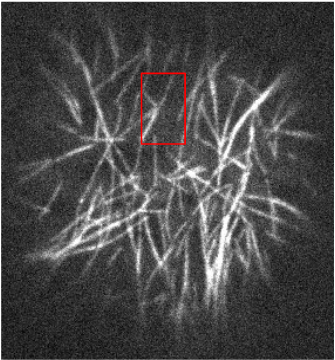
\includegraphics[scale=0.5]{imagenes/NoConsenso.png}
        \caption{Microt\'ubulos en planta {\it Marchantia}.\\Fuente: Paula Llanos}
        \label{fig:NoConsensoGeneral}
        \end{subfigure}  
        }
        &
        \multirow[c]{2}{*}[2cm]{
        \begin{subfigure}[t]{0.25\textwidth}
        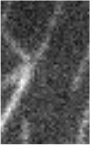
\includegraphics[]{imagenes/NoConsenso2.png}
        \caption{Secci\'on resaltada en rojo de \ref{fig:NoConsensoGeneral}}
        \label{fig:NoConsensoRect}
        \end{subfigure}
        }
        &
        \begin{subfigure}[t]{0.21\textwidth}
        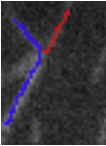
\includegraphics[scale=0.8]{imagenes/NoConsenso3.png}
        \caption{Opci\'on 1 de microt\'ubulos en \ref{fig:NoConsensoRect}}
        \label{fig:NoConsensoOpcion1}
        \end{subfigure} \\
        & &
        \begin{subfigure}[b]{0.21\textwidth}
        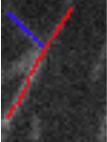
\includegraphics[scale=0.8]{imagenes/NoConsenso4.png}
        \caption{Opci\'on 2 de microt\'ubulos en \ref{fig:NoConsensoRect}}
        \label{fig:NoConsensoOpcion2}
        \end{subfigure} \\
    \end{tabular}
    
    \caption{Dificultad de individualizaci\'on que enfretan los expertos al analizar manualmente una imagen de filamentos, en particular, microt\'ubulos.}
    \label{fig:NoConsenso}
\end{figure*}

Un problema derivado de la resoluci\'on de una imagen en la que se observan filamentos yace en que 2 expertos pueden discernir al realizar una individualizaci\'on manual de filamentos, como se indica en las figuras \ref{fig:NoConsensoOpcion1} y \ref{fig:NoConsensoOpcion2}. Esta discrepancia implica que para algunos tipos de c\'elulas donde se observen filamentos no es posible conocer a priori del origen y el final de un filamento. Se presenta una dificultad adicional en la representaci\'on de un filamento en un grafo, ya que esta se basa en un conjunto de aristas adyacentes, denominadas caminos o recorridos, lo que lleva a tener un universo de hasta $n!$ posibles combinaciones en el espacio de soluciones en el que se busca un camino.


En base la gran cantidad de combinaciones posibles de caminos, el problema final en la individualizaci\'on de filamentos lo constituye la elecci\'on del subconjunto de caminos, que debe ser seleccionado entre el total de caminos que representan soluciones factibles. Esto implica que el problema no solo sea un problema combinatorial de generar soluciones factibles a partir del conjunto de aristas, sino que adem\'as debe considerar la discriminaci\'on entre estos para obtener el subconjunto de mayor calidad, pudiendo representarse como un problema de optimizaci\'on combinatorial.

Los problemas presentados se formalizan a continuaci\'on.

%problema previo
%presentar el problema previo, como un puente necesario en la automatizaci\'on de la extracci\'on,  para analizar un grafo que representa la red de filamentos, que de lo contrario tendria que ser realizado a mano, implicando que la persona realizando el análisis podría llevar a cabo la individualizaci\'on de filamentos en el mismo acto.

\section{Generaci\'on de un Grafo desde una Imagen}

La extracci\'on de un grafo a partir de una imagen, consiste en extraer un grafo $G = (V,E)$ de una imagen tal que $G$ sea un grafo simple, no dirigido, ponderado, conectado o desconectado, con o sin ciclos. Esto implica que exista a lo m\'as 1 arista por cada par de nodos adyacentes, prohibi\'endose la existencia de nodos conectados consigo mismos. Se definen los v\'ertices/nodos del grafo $G$ como $V(G)$ y las aristas de $G$ como $E(G)$. 
Que el grafo $G$ sea ponderado implica que para las aristas del grafo ($E(G)$), existen caracter\'isticas asociadas que se expresan como caracter\'isticas geom\'etricas, topol\'ogicas, espaciales y/u otras. Es importante evitar que $G$ sea un grafo completo, dado que con n nodos/v\'ertices $G$ llega a tener $\frac{n(n-1)}{2}$ aristas.
%$\forall e \in \quad E(G) \quad  \exists $ 

Como se menciona al inicio de este cap\'itulo, el ruido en una imagen y la resoluci\'on de la misma son aspectos que pueden perjudicar la obtenci\'on de un grafo a partir de una imagen. Mientras que el ruido ha sido estudiado en la literatura, el problema de resoluci\'on depende principalmente de la capacidad del microscopio que se utilice. El l\'imite m\'aximo de resoluci\'on, denominado $\frac{\lambda}{2}$, determina el tama\~no m\'inimo que 2 objetos que se encuentren juntos pueden tener para no observarse como un \'unico elemento. Lo anterior sucede para algunos tipos de filamentos como los microt\'ubulos que pueden medir tan solo 25 nan\'ometros, lo que se encuentra por debajo de $\frac{\lambda}{2}$ para diversos microscopios. 


La importancia del procedimiento de extraci\'on o generaci\'on de un grafo que representa una red de filamentos a partir de una imagen radica en que define la cantidad de informaci\'on disponible para llevar a cabo la individualizaci\'on de filamentos. A partir de una imagen es posible obtener una cantidad de caracter\'isticas de distinta \'indole, lo que permite en etapas posteriores clasificar de diversas formas nodos, aristas, de forma aislada o en conjuntos, efectivamente disminuyendo el espacio de b\'usqueda. Con las herramientas actuales disponibles en la literatura, es posible realizar la extracci\'on de una red de filamentos con algún nivel de informaci\'on como en \cite{xu2015soax}. Sin embargo, las transformaci\'on de aquella red a un grafo, as\'i como la incorporaci\'on de las caracter\'isticas y/o propiedades hacia el grafo son un procedimiento no automatizado, por lo que el esfuerzo que el experto debe realizar es cercano a individualizar los filamentos de manera manual.

A partir de las investigaciones en la literatura, es posible agrupar los m\'etodos para extraer la informaci\'on que permite la construcci\'on de un grafo a partir de una imagen, como lo son los nodos y las aristas, en dos conjuntos: Los que se basan en esqueletonizaci\'on\cite{lavado2018comparacion} y los que no. 

\subsection{Extracci\'on de un Grafo mediante Esqueletonizaci\'on}
\label{subsec:infoLossSkel}

%Que es la skeletonizacion y como extrae el grafo. Uso de liberia sknw
Los m\'etodos basados en esqueletonizaci\'on consisten primariamente en la reducci\'on de los p\'ixeles pertenecientes al plano de inter\'es o {\it foreground} en una imagen binaria, hasta formar una representaci\'on del objeto en la imagen de 1 p\'ixel de ancho. El proceso debe mantener la conectividad del objeto adelgazado y a su vez, reducir la dimensi\'on del objeto en la imagen para facilitar su an\'alisis\cite{saha2017skeletonization}. Un an\'alisis de los vecindarios de los p\'ixeles del esqueleto construido es una de las formas m\'as sencillas en que se puede distinguir si un p\'ixel representa un nodo o si es parte de un arista. Una librer\'ia que realiza tal an\'alisis es {\it skan}\cite{nunez2018new}, entregando estad\'isticas del grafo extra\'ido como largo promedio de una rama del esqueleto (equivalente a una arista del grafo), tipo de rama, curvatura de una rama, entre otras mediciones. Sin embargo, el formato de salida del grafo para esta herramienta corresponde a {\it Compressed sparse row} o CSR, lo que causa que un an\'alisis de mayor profundidad o el paso del grafo a una herramienta de individualizaci\'on de filamentos necesite de una librer\'ia adicional. 


Otra herramienta que realiza un an\'alisis similar para obtener un grafo a partir de un esqueleto es {\it sknw}, parte del framework {\it ImagePy}\cite{wang2018imagepy}. La diferencia propuesta por {\it sknw} radica en que se integra con la librer\'ia {\it NetworkX}\cite{hagberg2008exploring}, utilizando la estructura de datos para grafos que esta \'ultima posee para elegir entre m\'ultiples formatos de salida. Aquello otorga flexibilidad en la integraci\'on de herramientas que utilizan como base el grafo para realizar an\'alisis posteriores, como es el caso de la individualizaci\'on de filamentos.

% se puede extraer el skeleton con librerias en varios lenguajes, como octave, matlab o python (usando scipy). La opci\'on se encuentra en la secci\'on de herramientas morfol\'ogicasd de cada uno. De ahi al grafo, se puede utilizar un procedimiento que haga an\'alisis de vecindarios de p\'ixeles como \cite{qiu2014quantitative}

%problema de skeleton
Independiente de la herramienta usada para obtener la informaci\'on topol\'ogica de la c\'elula observada, el procedimiento de esqueletonizaci\'on puede sufrir de p\'erdida de informaci\'on, dado que mediante el o los pasos de adelgazamiento, puede existir p\'erdida de la informaci\'on de los vecinos de los p\'ixeles que conforman el esqueleto obtenido. Esta informaci\'on puede ser relativa a aspectos geom\'etricos como el ancho, o servir como los datos de entrada para calcular informaci\'on derivada mediante m\'etodos como {\it image moments}\cite{flusser2009moments}\cite{chaumette2004image}.

% mencionar superpixels y describir que son citando a 
Una forma de obtener la informaci\'on de vecindario mencionada es siguiendo la idea de agrupaci\'on de p\'ixeles similares o cercanos utilizada en superpixeles\cite{achanta2012slic}. Los algoritmos de generaci\'on de superpixeles juntan conjuntos de p\'ixeles para obtener nuevas unidades at\'omicas sobre las cuales se realiza el an\'alisis, reduciendo la complejidad de este. El prop\'osito de basarse en la idea de superpixeles y no en el concepto de forma completa se fundamenta en que no se busca generar una segmentaci\'on acabada, sino que poder asociar los superpixeles con los nodos y aristas que resultan al transformar el esqueleto a un grafo. Para aquello, es s\'olo necesario realizar una agrupaci\'on gruesa utilizando criterios de tama\~no m\'aximo de un superpixel, dado que en im\'agenes binarias o en escala de grises el uso de criterios de similaridad seg\'un el valor de cada p\'ixel puede llevar a obtener un n\'umero muy bajo de superpixeles, ocasionando que m\'ultiples nodos y/o aristas se refieran al mismo superpixel. El detalle de la implementaci\'on de la agrupaci\'on de p\'ixeles y su asociaci\'on con los nodos se encuentra en la secci\'on \ref{sec:superpixels}.


\subsection{Obtenci\'on de Informaci\'on Adicional}

Para dar uso a la informaci\'on recuperada de acuerdo a lo expresado en la secci\'on \ref{subsec:infoLossSkel}, se analizaron diversos filtros \'utiles para describir estructuras alargadas, como {\it Gabor}, {\it Anistropic Diffusion} y Frangi para {\it Veselness}. El filtro Frangi para {\it Veselness}\cite{frangi1998multiscale}\cite{fu2018frangi}, cuantifica cuan alargada es una estructura ({\it veselness value}), en base a los valores y vectores propios de la matriz Hessiana (ecuaci\'on \eqref{eq:HessianMat}) posterior a la aplicaci\'on de uno o varios filtros Gaussianos para suavizar una imagen. Este filtro es utilizado en la detecci\'on de estructuras alargadas como arterias y venas, pudiendo replicarse parcialmente mediante el an\'alisis de p\'ixeles con {\it image moments}\cite{flusser2009moments}. La posibilidad de replicar el filtro de Frangi, sin necesidad de configurar par\'ametros, es lo que llev\'o a elegirlo por sobre las otras opciones.

\begin{equation}
    \label{eq:HessianMat}
    H = \begin{bmatrix}
        H_{xx} & H_{xy} \\
        H_{xy} & H_{yy} 
        \end{bmatrix}
\end{equation}

Una respuesta de {\it veselness value} que denota una estructura alargada se obtiene si los 2 eigenvalores, $\lambda_1$ y $\lambda_2$ ($|\lambda_2| \geq |\lambda_1|$) satisfacen $|\lambda_1| \approx 0 $ y $|\lambda_2| \gg |\lambda_1|$. Los eigenvalores se obtienen mediante la ecuaci\'on \ref{eq:lambdaFrangi}.

\begin{equation}
    \label{eq:lambdaFrangi}
    \lambda_{1,2} = \dfrac{(H_{xx} + H_{yy}) \pm \sqrt{(H_{xx} - H_{yy})^{2} + 4\cdot H_{xy}^{2}     } }{2}
\end{equation}

Otra forma de obtener los valores de lambda de la ecuaci\'on \ref{eq:lambdaFrangi} es utilizando los {\it central image moments} o momentos centrales, que derivan de los {\it raw image moments} obtenidos en el segundo paso la herramienta para recuperar informaci\'on presentada en la secci\'on \ref{subsec:infoLossSkel}. Se define un {\it raw image moment} de orden $p+q$ para una imagen en la ecuaci\'on \eqref{eq:rawImageMoment}, donde $f(x,y)$ corresponde a la intensidad de la imagen en un punto (x,y). El {\it raw moment} $M_{00}$ refleja la "masa" de la imagen, correspondiendo al \'area o volumen si se trata de una imagen binaria. 

Para el c\'alculo de los momentos centrales se agregan los componentes del centroide, $\overline{x}$ e $\overline{y}$, basados en los {\it raw moments}, como indican las ecuaciones \eqref{eq:avgFromRawMomts} y \eqref{eq:centralImageMoment}.

\begin{subequations}
\begin{equation}
    \label{eq:rawImageMoment}
    M_{pq} = \sum\limits_{x} \sum\limits_{y} x^p \cdot y^q \cdot f(x,y)
\end{equation}
\begin{equation}
    \label{eq:avgFromRawMomts}
    \overline{x} = \frac{M_{10}}{M_{00}}, \quad
    \overline{y} = \frac{M_{01}}{M_{00}}
\end{equation}
\begin{equation}
    \label{eq:centralImageMoment}
    \mu_{pq} = \sum\limits_{x} \sum\limits_{y} (x - \overline{x})^{p} \cdot (y - \overline{y})^{q} \cdot f(x,y)
\end{equation}
\end{subequations}

As\'i, es posible construir una matriz de covarianza, equivalente a la matriz hessiana en la ecuaci\'on \eqref{eq:HessianMat}, utilizando los momentos centrales de segundo orden, $\mu_{20}$, $\mu_{02}$ y $\mu_{11}$ divididos por el momento central de orden cero $\mu_{00}$ (ecuaciones \eqref{eq:mu20}, \eqref{eq:mu02} y \eqref{eq:mu11}), obteniendo los eigenvalores mediante la ecuaci\'on \eqref{eq:lambdaMoments}.

\begin{subequations}
\begin{align}
    \mu_{20}^{\prime} &= \frac{\mu_{20}}{\mu_{00}} = \frac{M_{20}}{M_{00}} - \overline{x}^{2} \label{eq:mu20} \\
    \mu_{02}^{\prime} &= \frac{\mu_{02}}{\mu_{00}} = \frac{M_{02}}{M_{00}} - \overline{y}^{2} \label{eq:mu02} \\
    \mu_{11}^{\prime} &= \frac{\mu_{11}}{\mu_{00}} = \frac{M_{11}}{M_{00}} - \overline{x}\cdot\overline{y} \label{eq:mu11}
\end{align}

\begin{equation}
    \label{eq:covMatLambda}
    cov[f(x,y)] = \begin{bmatrix}
        \mu_{20}^{\prime} & \mu_{11}^{\prime} \\
        \mu_{11}^{\prime} & \mu_{02}^{\prime} 
        \end{bmatrix}
\end{equation}

\begin{equation}
    \label{eq:lambdaMoments}
    \lambda_{1,2} = \dfrac{(\mu_{20}^{\prime} + \mu_{02}^{\prime}) \pm \sqrt{(\mu_{20}^{\prime} - \mu_{02}^{\prime})^{2} + 4\cdot \mu\prime_{11}^{2} }}{2}
\end{equation}
\end{subequations}

Con los valores de $\lambda$, es posible calcular caracter\'isticas de una estructura alargada como su excentricidad o su eje principal de inercia. Estas medidas pueden ayudar a mejorar la clasificaci\'on de segmentos del grafo durante la identificaci\'on de filamentos.


% informacion geometrica mediante calculo de angulos entre aristas
Un manera adicional de generar informaci\'on que facilite la discriminaci\'on de secciones del grafo es a trav\'es del c\'alculo de los \'angulos entre las aristas del grafo. Esto se relaciona a criterio de rectitud que tienen los filamentos, que var\'ia dependiendo de la c\'elula a la que pertenezca. Este comportamiento de los filamentos permite delimitar el \'angulo m\'aximo que 2 aristas contiguas pueden tener para ser considerados parte del mismo filamento, denomin\'andose este umbral como $Max\_Angle$. Cualquier valor por sobre $Max\_Angle$ permite descartar de forma absoluta esa combinanci\'on de aristas para un mismo filamento. 


A su vez, este criterio posee un segundo umbral, definido como $\theta$  que define el \'angulo m\'aximo bajo el que se considera que 2 aristas contiguas respetan con certeza la rectitud necesaria para formar parte del mismo filamento. Es decir, si 2 aristas contiguas forman un \'angulo en el rango $[0, \theta]$, deben ser parte del mismo filamento. El rango entre ambos umbrales, $]\theta, Max\_Angle]$ delimita los pares de aristas que a priori no representan combinaciones que respetan el criterio de rectitud, pero cuya explicaci\'on puede encontrarse en variaciones inducidas durante la extracci\'on del grafo desde la imagen, por lo que es necesario incorporar la exploraci\'on de estos pares de aristas.


Finalmente, para el caso de los nodos, el an\'alisis del grado de cada uno permite identificar la existencia de ciclos\cite{wilson1979introduction} en un filamento. La propiedad de un filamento de poder o no tener un ciclo es informaci\'on disponible priori que depende del tipo de c\'elula observada, permitiendo limitar posibles asociaciones entre nodos. En el caso particular de no permitir ciclos, un filamento no podr\'ia pasar m\'as de una vez por cada nodo que lo conforma. 

%se destaca dentro de los criterios: busca evitar perder información de la imagen/ampliar la informacion así como tener un costo computacional bajo, en conjunto con disminuir la interacción del usuario. 


% ambas opciones generan degeneraciones/deformaciones q afectan
\section{Exploraci\'on del Espacio de Soluciones}

La b\'usqueda de conjuntos de nodos o aristas adyacentes (denominados caminos) en un grafo, para individualizar uno o m\'as filamentos, constituye un espacio de soluciones que no es posible de recorrer en tiempo polinomial, dado que sin restricciones las combinaciones crecen exponencialmente\cite{buchin2007number}\cite{biswas2012hamiltonian}. Un planteamiento similar a lo anterior es el {\it Path Cover Problem} o PCP, en el que se descompone un grafo dirigido en caminos con el objetivo de obtener un conjunto de caminos. Cada nodo o arista debe pertenecer exactamente a un camino y los caminos pueden comenzar o terminar en cualquier parte del grafo.

En el caso de la individualizaci\'on de filamentos, es necesario que la definici\'on del problema considere como v\'alidos caminos que representen los casos de filamentos con o sin ciclos, as\'i como superposici\'on y/o cruce. Lo anterior impide forzar la pertenencia de un nodo o arista a un s\'olo camino. 

% explicar define: como lo hace define? y como se observa la potencial perdida de soluciones factibles al usar un solo criterio
La investigaci\'on de \cite{breuer2015define}, denominada {\tt DeFiNe}, descrita brevemente en el cap\'itulo \ref{chap:stateoftheart} presenta el {\it Filament Cover Problem} o FCP como una extensi\'on del PCP, flexibilizando la pertenencia de cada arista a al menos un camino. Adem\'as plantean como funci\'on objetivo la minimizaci\'on de la diferencia de la homogeneidad (aspereza) entre las aristas que componen un camino. Para acotar el espacio de soluciones, los autores de DeFiNe proponen 2 heur\'isticas fundamentando que el FCP en \'arboles en vez de grafos es soluble en tiempo polinomial. Aquello se basa en lo definido por \cite{lin2006vertex} que indica que para un problema de {\it covering}, existe un {\it Set System} $(S,C)$, donde S es el conjunto total y finito de sets, y C es un conjunto de subsets pertenecientes a S. En el caso espec\'ifico del {\it Minimum Set Cover} (MSC), el objetivo es encontrar un subconjunto $C'$ de $C$ tal que cada elemento de $S$ pertenezca al menos 1 vez a uno de los miembros de $C'$.

%Un grafo completamente conectado puede tener n(n-1)/2 aristas, lo que para un n muy grande puede implicar un costo computacional alto
%A su vez, otro motivo para evitar que $G$ sea un grafo completo radica en que para los filamentos observados en la naturaleza no es una condici\'on comun... no encuentro la fuente de esto

%Denominamos todas estas opciones de caminos como el conjunto $P$, del cual debemos extraer un subconjunto $P'$ mediante una estrategia que permita realizar esto en tiempo polinomial independientemente de la cantidad de aristas del grafo.

Para un {\it set system} $(S,C)$ que pueda ser representando por un \'arbol $T$, es posible mutar la definici\'on de $S$ al conjunto de nodos que componen un grafo $G$, y a su vez, hacer que cada subset $c \in C$ represente un camino simple en $G$. Un camino simple es equivalente a un \'arbol simple (2 nodos son unidos por a lo m\'as 1 arista) y ac\'iclico.


Se destaca en \cite{lin2006vertex} que no todos los caminos simples de $G$ est\'an representados en $C$. Esta representaci\'on de {\it covering} de caminos, o {\it Path Cover}, es denominada {\it Vertex Covering by Paths on Graphs} (VcpG) y difiere de un {\it Path Cover} tradicional al permitir caminos que compartan nodos. Luego, para el caso de \'arboles, VcpG se renombra a VcpT ({\it Vertex Covering by Paths on Trees}), permitiendo el reemplazo de nodos por aristas sin generar cambios significativos en el planteamiento del problema. Esta modificaci\'on de nodos a aristas se denomina EcpT ({\it Edge Covering by Paths on Trees}). %recordar mas adelante como posible perdida de soluciones factibles


Lo anterior establece el fundamento para que los autores de DeFiNe\cite{breuer2015define} utilicen EcpT como base, teniendo un m\'aximo de caminos $n(n)-1/2 = \mathcal{O}(n^{2})$, con una complejidad $\mathcal{O}(n^{4})$ para obtener esos caminos. La obtenci\'on de caminos a partir de un \'arbol $T$ que contiene los nodos del grafo $G$ se realiza mediante la divisi\'on continua del \'arbol en m\'ultiples bosques, hasta que los bosques resultantes sean s\'olo caminos simples. Sin embargo, los caminos resultantes no comparten nodos o aristas, es decir, no se superponen. Para solucionar aquello manteniendo la resoluci\'on del FCP en tiempo polinomial, se agrega en DeFiNe el par\'ametro $k$, que define el n\'umero m\'aximo de superposiciones de caminos en una arista. La complejidad con el nuevo par\'ametro queda como $\mathcal{O}(n^{2k+2})$.


%aca entran las formas de obtener esos arboles simples y bosques, con las heuristicas de define
Dado que el conjunto total de caminos en un grafo, definido como $P$, no es calculables en tiempo polinomial, DeFine propone 2 heur\'isticas para construir \'arboles de los cuales se puedan extraer un conjunto representativo de caminos simples, definidos como $P'$. Cada una de las heur\'isticas, {\it BFS} y {\it RMST}, explicadas en el cap\'itulo \ref{chap:stateoftheart}, proveen un conjunto $P'$, al que se le aplica la funci\'on objetivo, para encontrar los miembros de $p \in P'$ que mejor minimicen la diferencia de homogeneidad en sus caminos. La restricci\'on de lo anterior es que cada arista del grafo pertenezca a lo menos a un camino. 

%\begin{equation}
%p = (e_1, e_2,..., e_n)\\
%p = ((v_1,v_2), (v_2,v_4),..., (v_n-1,v_n))
%\label{eq:path}
%\end{equation}

% Comparándose con define, Problema 1 caminos validos no llegan a P'

La generaci\'on del conjunto $P'$ planteado en DeFiNe puede llevar a excluir caminos v\'alidos al realizar la representaci\'on de un {\it set system} mediante un \'arbol, o al utilizar una sola propiedad asociada a un filamento en una de sus heur\'isticas. 


El presente trabajo plantea en el cap\'itulo \ref{sec:modeloOpti} un modelo de optimizaci\'on que permite generar caminos utilizando m\'as de una propiedad asociada a un filamento o al grafo que representa la red de filamentos. Esto permite individualizar filamentos en casos de superposici\'on, cruce o discriminando si el filamento puede tener o no ciclos. Adem\'as se presentan diversas heur\'isticas para reducir el tama\~no del espacio de soluciones.

%Ejemplo camino verde en Spinning Marchantia (imagenes)


